\chapter{Contour of Layers \label{contour_of_layers}}

\section{Introduction}
Despite any optimisations, users may still feel unsatisfied because ambiguous information such as artefacts and depth ambiguity could be introduced in volume rendering.
NPR techniques are one means of providing insight into volume data in a similar way that medical illustrations depict the important details of anatomical structures \cite{svakhine_illustration-inspired_2009}. 
Therefore, illustrative depictions are introduced in our approach to improve the expressiveness of the visualization. In order to improve the clarity of contours, we present two approaches to outline the contour of parts of the volume. These methods provide effects similar to two-level volume rendering techniques \cite{hauser_two-level_2001} \cite{corcoran_perceptual_2010}.

\section{Contour of Layers in 1D Transfer Function Domains}
The contour outlining approach described in this section is an image space addition to volume rendering. This approach involves user selection of transfer function features and composition of partial renderings in the image space. A transfer function feature is a group of three adjacent control points with the same colour corresponding to an intensity range.
We use the rendered images (\ref{fig:multiple_nucleon_with_contour}) of the nucleon data set to demonstrate the pipeline of this method.

The three transfer function features \ref{fig:tf_nucleon_2} are selected separately to perform a volume rendering of the nucleon data set. Then edge detection (which uses the Sobel operator) is performed on each of the three resulting images to obtain the contour of the selected features (or a layer) of the transfer function. Subsequently, the contours of the three layers are composited together, as shown in \ref{fig:nucleon_threshold_contour}. Finally, the contours are composited back to the original rendering in \ref{fig:nucleon_original} and yield the result in \ref{fig:nucleon_with_contour}.

This approach is straightforward but it can only generate contours which are distinguishable in 1D transfer function domain, i.e. where the transfer function features do not overlap.
Figure~\ref{fig:multiple_Engine_with_contour} and Figure~\ref{fig:multiple_VisMale_spectrum_4_balance_1000_threshold_contour} show two sets of resulting images.

In these results, transfer functions are optimized before applying the contour outlining approach. For the VisMale data set, region-based optimization is also performed (Figure~\ref{fig:VisMale_spectrum_8_balance_1000_region_1000}) with the region selected from a partial rendering of the skull (Figure~\ref{fig:VisMale_spectrum_8_balance_1000_peeled_selection}). The selection on the partial rendering excludes the surrounding material, so that the skull will be further enhanced in the resulting transfer function.

\begin{figure}
	\centering
	\begin{subfigure}[b]{0.25\textwidth}
		\centering
		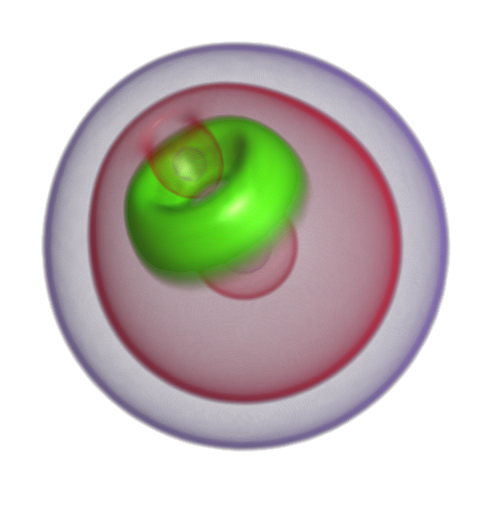
\includegraphics[width=\textwidth]{nucleon_original.png}
		\caption{A rendered image of the nucleon data set}
		\label{fig:nucleon_original}
	\end{subfigure}%
	\begin{subfigure}[b]{0.25\textwidth}
		\centering
		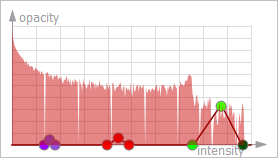
\includegraphics[width=\textwidth]{tf_nucleon.png}
		\caption{Set each control as a layer}
		\label{fig:tf_nucleon_2}
	\end{subfigure}%
	\begin{subfigure}[b]{0.25\textwidth}
		\centering
		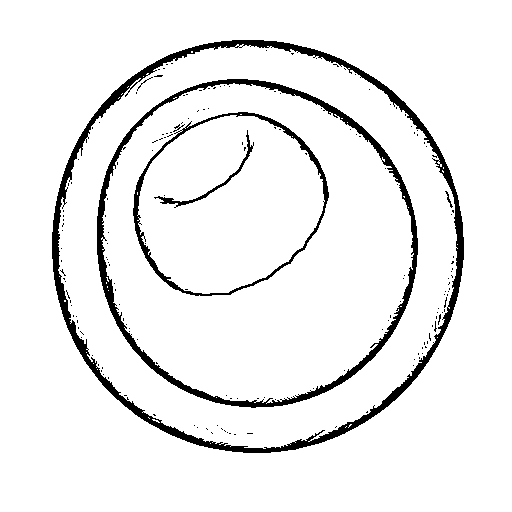
\includegraphics[width=\textwidth]{nucleon_threshold_contour.png}
		\caption{The contours of the three layers blended together}
		\label{fig:nucleon_threshold_contour}
	\end{subfigure}%
	\begin{subfigure}[b]{0.25\textwidth}
		\centering
		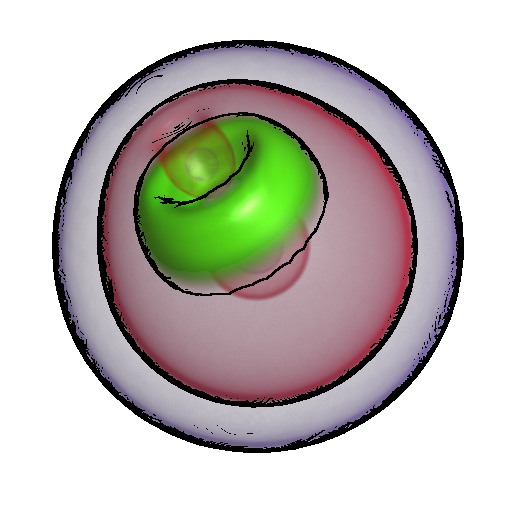
\includegraphics[width=\textwidth]{nucleon_with_contour.png}
		\caption{The rendered image blended with contour}
		\label{fig:nucleon_with_contour}
	\end{subfigure}        
	\caption{The nucleon data set}\label{fig:multiple_nucleon_with_contour}
\end{figure}

%\subsection{Results}

\begin{figure}
	\centering
	\begin{subfigure}[b]{0.24\textwidth}
		\centering
		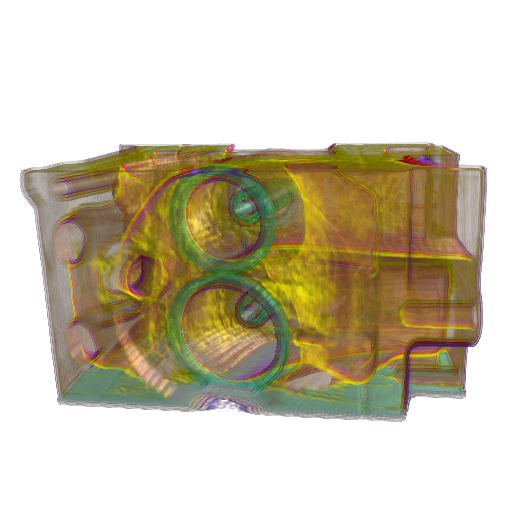
\includegraphics[width=\textwidth]{Engine.png}
		\caption{A rendered image of the engine block data set}
		\label{fig:Engine}
	\end{subfigure}~
	\begin{subfigure}[b]{0.24\textwidth}
		\centering
		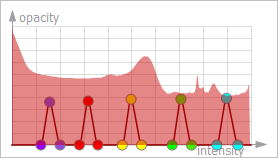
\includegraphics[width=\textwidth]{tf_Engine.png}
		\caption{The initial transfer function}
		\label{fig:tf_Engine}
	\end{subfigure}~
	\begin{subfigure}[b]{0.24\textwidth}
		\centering
		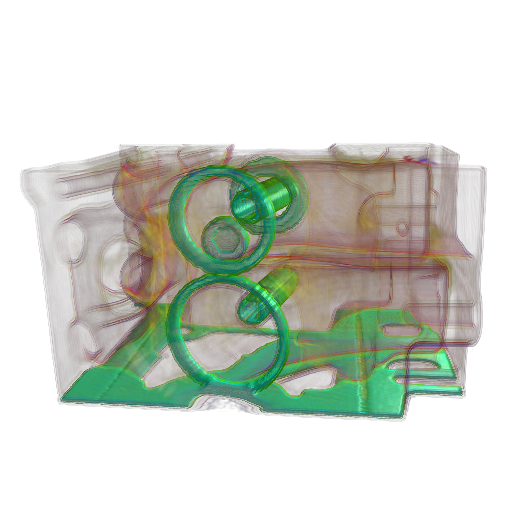
\includegraphics[width=\textwidth]{Engine_balance_300.png}
		\caption{After balancing opacity}
		\label{fig:Engine_balance_300}
	\end{subfigure}~
	\begin{subfigure}[b]{0.24\textwidth}
		\centering
		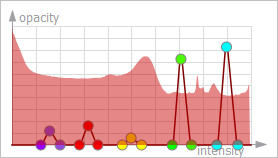
\includegraphics[width=\textwidth]{tf_Engine_balance_300.png}
		\caption{The optimised transfer function}
		\label{fig:tf_Engine_balance_300.png}
	\end{subfigure}
	~ %add desired spacing between images, e. g. ~, \quad, \qquad etc.
	%(or a blank line to force the subfigure onto a new line)
	\begin{subfigure}[b]{0.24\textwidth}
		\centering
		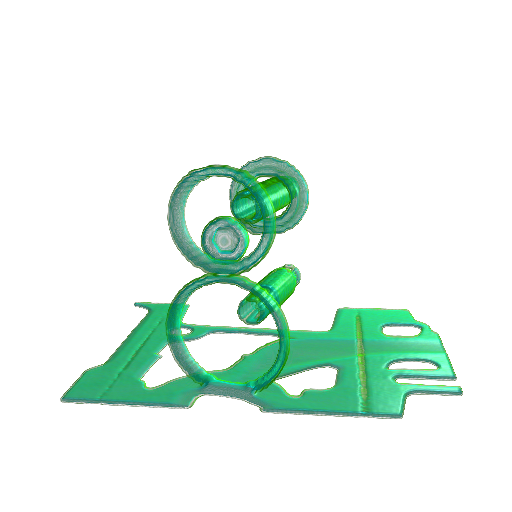
\includegraphics[width=\textwidth]{Engine_balance_300_threshold.png}
		\caption{After thresholding}
		\label{fig:Engine_balance_300_threshold}
	\end{subfigure}~    
	\begin{subfigure}[b]{0.24\textwidth}
		\centering
		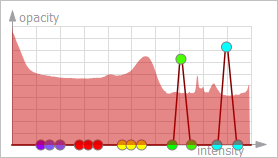
\includegraphics[width=\textwidth]{tf_Engine_balance_300_threshold.png}
		\caption{Set the opacity of a control point to zero if it is below the threshold}
		\label{fig:tf_Engine_balance_300_threshold.png}
	\end{subfigure}~
	\begin{subfigure}[b]{0.24\textwidth}
		\centering
		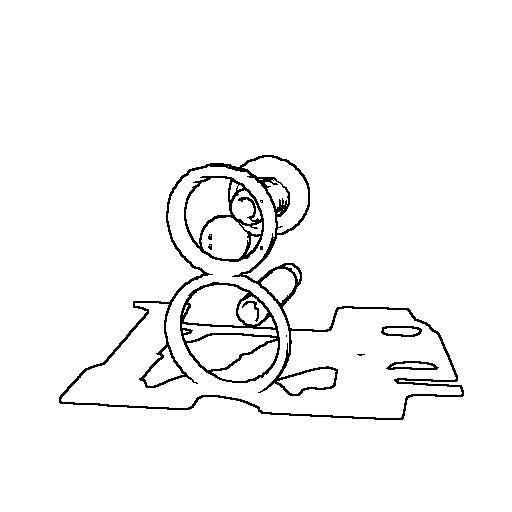
\includegraphics[width=\textwidth]{Engine_balance_300_threshold_contour.png}
		\caption{The contour extracted from \ref{fig:tf_Engine_balance_300_threshold.png}}
		\label{fig:Engine_balance_300_threshold_contour}
	\end{subfigure}~
	\begin{subfigure}[b]{0.24\textwidth}
		\centering
		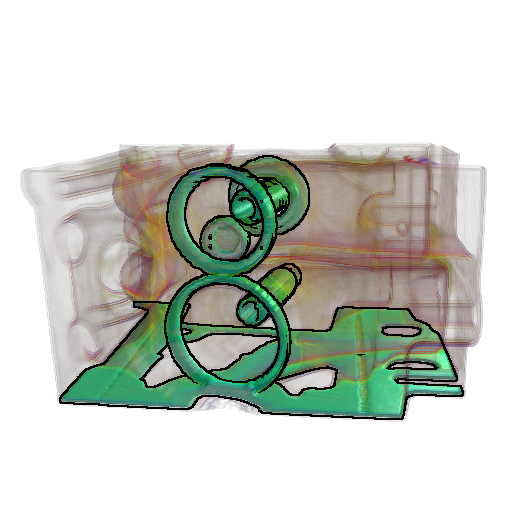
\includegraphics[width=\textwidth]{Engine_with_contour.png}
		\caption{Blend the contour (\ref{fig:Engine_balance_300_threshold_contour}) with the rendered image in \ref{fig:Engine_balance_300}}
		\label{fig:Engine_with_contour}
	\end{subfigure}
	\caption{The engine block data set}
	\label{fig:multiple_Engine_with_contour}
\end{figure}

\begin{figure}
	\centering
	\begin{subfigure}[b]{0.24\textwidth}
		\centering
		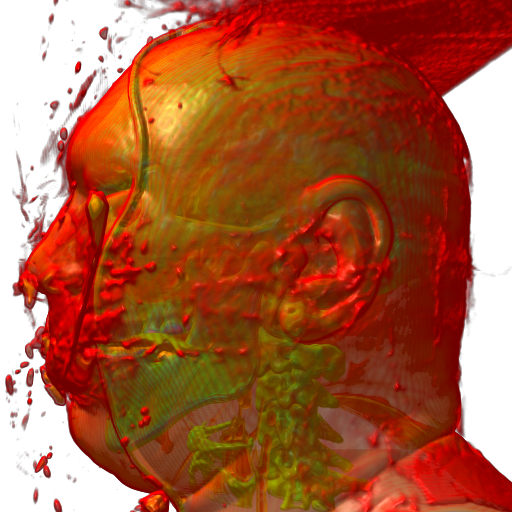
\includegraphics[width=\textwidth]{VisMale_spectrum_8.png}
		\caption{The VisMale data set}
		\label{fig:VisMale_spectrum_8}
	\end{subfigure}~
	\begin{subfigure}[b]{0.24\textwidth}
		\centering
		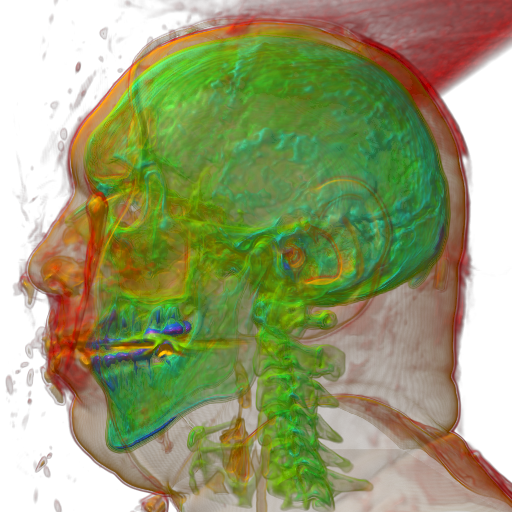
\includegraphics[width=\textwidth]{VisMale_spectrum_8_balance_1000.png}
		\caption{After global optimization}
		\label{fig:VisMale_spectrum_8_balance_1000}
	\end{subfigure}~
	\begin{subfigure}[b]{0.24\textwidth}
		\centering
		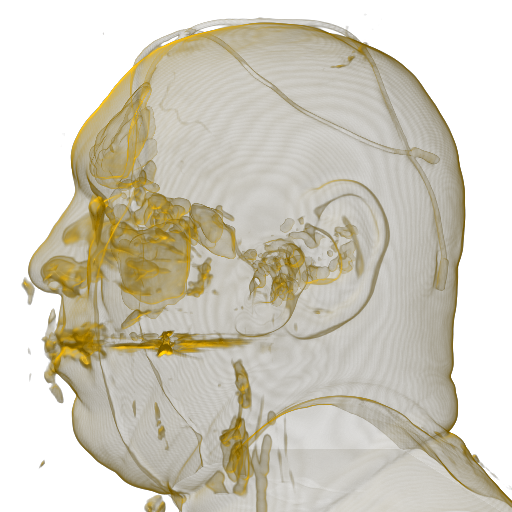
\includegraphics[width=\textwidth]{VisMale_spectrum_8_balance_1000_threshold.png}
		\caption{Render only one set of control points in the transfer function}
		\label{fig:VisMale_spectrum_8_balance_1000_threshold}
	\end{subfigure}~
	\begin{subfigure}[b]{0.24\textwidth}
		\centering
		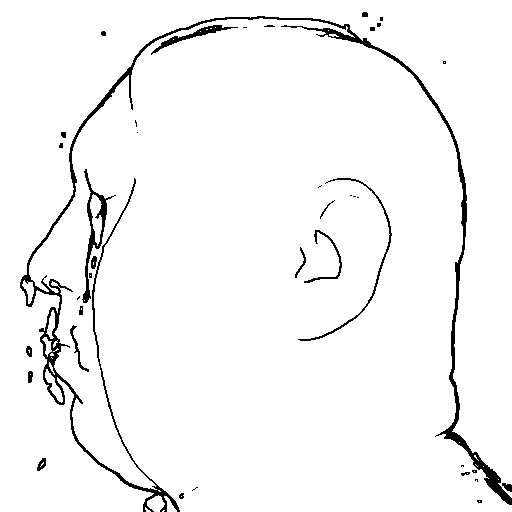
\includegraphics[width=\textwidth]{VisMale_spectrum_8_balance_1000_threshold_contour.png}
		\caption{Edge detection is performed on \ref{fig:VisMale_spectrum_8_balance_1000_threshold}}
		\label{fig:VisMale_spectrum_8_balance_1000_threshold_contour}
	\end{subfigure}
	\begin{subfigure}[b]{0.24\textwidth}
		\centering
		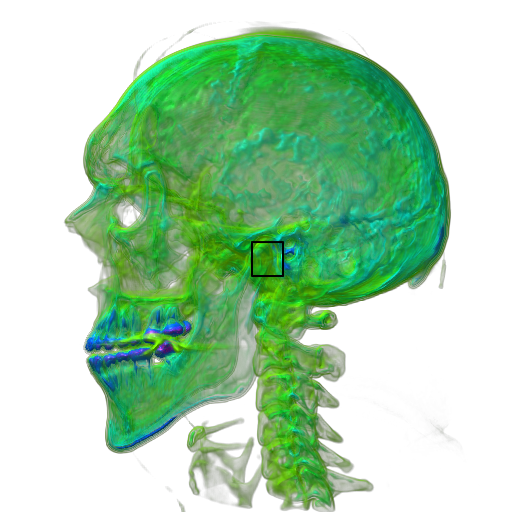
\includegraphics[width=\textwidth]{VisMale_spectrum_8_balance_1000_peeled_selection.png}
		\caption{Selection (the black rectangle) on a partial rendering to avoid selecting the outside layer}
		\label{fig:VisMale_spectrum_8_balance_1000_peeled_selection}
	\end{subfigure}~
	\begin{subfigure}[b]{0.24\textwidth}
		\centering
		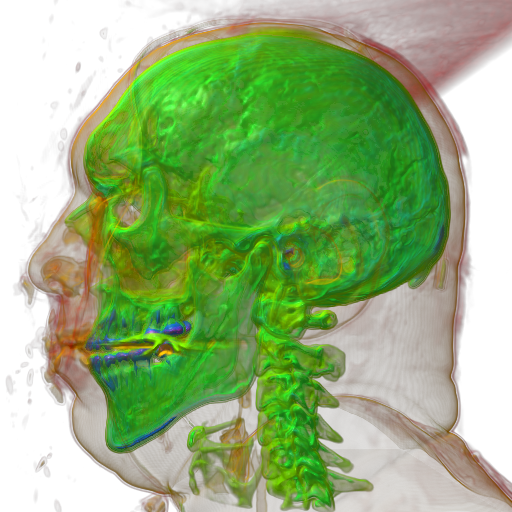
\includegraphics[width=\textwidth]{VisMale_spectrum_8_balance_1000_region_1000.png}
		\caption{Region-based optimization}
		\label{fig:VisMale_spectrum_8_balance_1000_region_1000}
	\end{subfigure}~
	\begin{subfigure}[b]{0.24\textwidth}
		\centering
		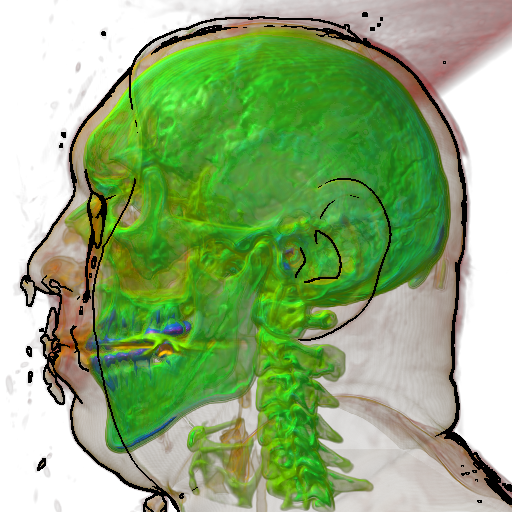
\includegraphics[width=\textwidth]{VisMale_spectrum_8_balance_1000_region_1000_threshold_contour_combined.png}
		\caption{The edge is combined}
		\label{fig:VisMale_spectrum_8_balance_1000_region_1000_threshold_contour_combined}
	\end{subfigure}~
	\begin{subfigure}[b]{0.24\textwidth}
		\centering
		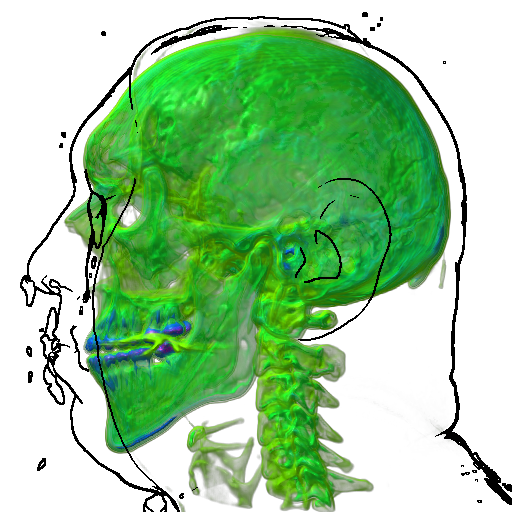
\includegraphics[width=\textwidth]{VisMale_spectrum_8_balance_1000_region_1000_peeled_threshold_contour_combined.png}
		\caption{The edge is combined and the outside layer is removed}
		\label{fig:VisMale_spectrum_8_balance_1000_region_1000_peeled_threshold_contour_combined}
	\end{subfigure}
	\caption{The VisMale data set}\label{fig:multiple_VisMale_spectrum_4_balance_1000_threshold_contour}
\end{figure}

%\begin{figure}
%        \centering
%        \begin{subfigure}[b]{0.4\textwidth}
%                \centering
%                \includegraphics[width=\textwidth]{VisMale7_region_selection2_150_squared_distance.png}
%                \caption{A rendered image of the VisMale data set}
%                \label{fig:VisMale7_region_selection2_150_squared_distance}
%        \end{subfigure}%
%        ~ %add desired spacing between images, e. g. ~, \quad, \qquad etc.
%          %(or a blank line to force the subfigure onto a new line)
%        \begin{subfigure}[b]{0.4\textwidth}
%                \centering
%                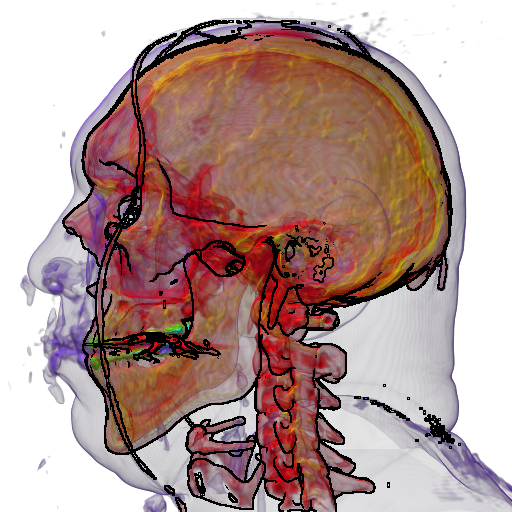
\includegraphics[width=\textwidth]{VisMale_with_contour.png}
%                \caption{The image blended with contour}
%                \label{fig:VisMale_with_contour}
%        \end{subfigure}
%        \caption{The VisMale data set}\label{fig:multiple_VisMale_with_contour}
%\end{figure}%
%\begin{figure}
%        \centering
%        \begin{subfigure}[b]{0.49\textwidth}
%                \centering
%                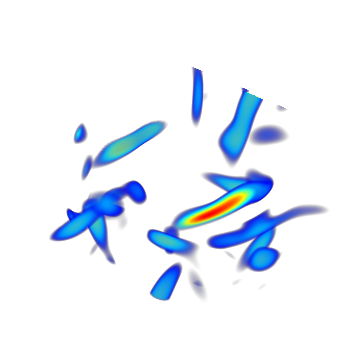
\includegraphics[width=\textwidth]{vortex_original_cr.png}
%                \caption{A rendered image of the vortex data set}
%                \label{fig:vortex_original}
%        \end{subfigure}%
%        ~ %add desired spacing between images, e. g. ~, \quad, \qquad etc.
%          %(or a blank line to force the subfigure onto a new line)
%        \begin{subfigure}[b]{0.49\textwidth}
%                \centering
%                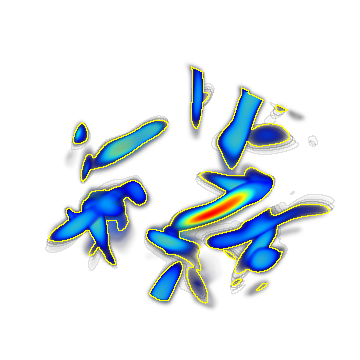
\includegraphics[width=\textwidth]{vortex_with_contour_cr.png}
%                \caption{The image with contour lines}
%                \label{fig:vortex_with_contour}
%        \end{subfigure}
%        \caption{The vortex data set}\label{fig:multiple_vortex_with_contour}
%\end{figure}

\section{Contour of Layers in Multidimensional Transfer Function Domains}
%Boundary regions between areas of relatively homogeneous material are believed to be critical in depicting structures. We examine existing boundary exploration techniques and propose a novel diagram to depict the boundary regions in volume data. This diagram provides useful information to guide the design of effective transfer functions in order to visualize structures in volume data.

%\subsubsection{Introduction}
In volume visualization, boundary regions between areas of relatively homogeneous material (i.e. different areas that are homogeneous within their own) are believed to be critical in depicting structures. Multidimensional transfer functions have proven to be an effective means of extracting materials and their boundaries for both scalar and multivariate data \cite{park_multi-dimensional_2004} \cite{maciejewski_structuring_2009}.

Classification and segmentation of volume data are challenging problems in volume visualization. Researchers have proposed a variety of approaches to tackle the problems.
%Several methods have been proposed to identify boundary regions in volume data.
Kindlmann and Durkin \cite{kindlmann_semi-automatic_1998} introduced the boundary model which consists of intensity, gradient magnitude and second directional derivative along the gradient direction.
Based on this idea, Kniss et al. \cite{kniss_multidimensional_2002} presented a set of manipulation widgets to specify multidimensional transfer functions (Figure~\ref{fig:kniss_multidimensional_2002_a} and Figure~\ref{fig:kniss_multidimensional_2002_b}).
Serlie et at. \cite{serlie_computed_2003} presented a three-material transition model that allows proper classification of transitions between three materials: gas, tissue and tagged material in CT volume data. Later, Sereda et al. \cite{sereda_visualization_2006} proposed the LH Histogram to identify the materials that form the boundaries (Figure~\ref{fig:sereda_visualization_2006}), where the L and H values are the lowest and highest intensity of the two-material transition model.

\begin{figure}
	\centering
	\begin{minipage}{.33\textwidth}
		\centering
		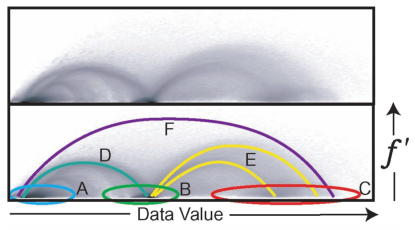
\includegraphics[width=1\textwidth]{kniss_multidimensional_2002_a.png}
		\caption{\cite{kniss_multidimensional_2002}}
		\label{fig:kniss_multidimensional_2002_a}
	\end{minipage}%
	\begin{minipage}{.33\textwidth}
		\centering
		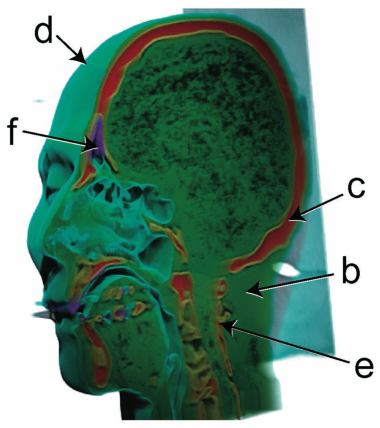
\includegraphics[width=1\textwidth]{kniss_multidimensional_2002_b.png}
		\caption{\cite{kniss_multidimensional_2002}}
		\label{fig:kniss_multidimensional_2002_b}
	\end{minipage}
	\begin{minipage}{.33\textwidth}
		\centering
		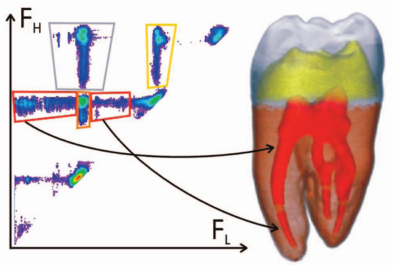
\includegraphics[width=1\textwidth]{sereda_visualization_2006.png}
		\caption{\cite{sereda_visualization_2006}}
		\label{fig:sereda_visualization_2006}
	\end{minipage}
\end{figure}

\subsection{Classification of Volume Data \label{classification_of_boundaries}}
We have proposed a clustering approach and implemented two other gradient-based methods for classification of voxels and plan to utilize these methods to guide the design of transfer functions and non-photorealistic rendering (NPR) techniques.

We proposed a clustering approach based on intensity, gradient magnitude and second order derivative magnitude of voxels for classification of volume data. Figure~\ref{fig:intensity_gradient_second_derivative} shows the clustering result of voxels in the 3D transfer function domain of intensity, gradient magnitude and second derivatives. The voxels are classified into clusters with the k-means clustering algorithm. Each cluster is assigned a different colour and the squares represent the centroids of the clusters.

We have implemented a 2D transfer function of intensity and gradient magnitude, as shown in Figure~\ref{fig:gradient_intensity}. The voxels are scattered on this 2D diagram based on their intensities and gradient magnitudes and are coloured according to their gradient directions.
Figure~\ref{fig:gradient_intensity_spatial} is the same 2D transfer function, but the voxels are coloured according to their spatial positions (similar to the idea in \cite{roettger_spatialized_2005}). The nucleon data set is used to draw the diagrams.

In addition, we have also implemented the LH Histogram \cite{sereda_visualization_2006}. The $ F_{L} $ (lower intensity) and $ F_{H} $ (higher intensity) in the LH Histogram are the lowest and highest intensity of the two-material transition model.
The LH Histogram can be constructed as follows.
For each voxel of the volume, we first determine if it lies on a boundary by looking at the if the gradient magnitude is less than or equal to a pre-defined threshold. If the voxel does not lie on a boundary, its $ F_{L} $ and $ F_{H} $ are both set as its intensity. If the voxel lies on a boundary (its gradient magnitude is greater than the threshold), a path is tracked by integrating the gradient field in both directions. The integration stops when we reach a large constant area, a local minimum or a inflection point. Figure~\ref{fig:lh_histogram} shows a LH Histogram with a colour scheme based on voxel intensity.
%Figure~\ref{fig:lh_histogram} and Figure~\ref{fig:lh_histogram_spatial} are two LH Histograms with different colour scheme. The former assigns colours based on voxel intensity and the latter assigns colours based on voxel spatial positions.

\begin{figure}
	\centering
	\begin{minipage}{.24\textwidth}
		\centering
		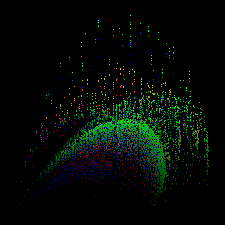
\includegraphics[width=1\textwidth]{gradient_intensity.png}
		\caption{A plot of gradient and intensity (x-axis (horizontal) for intensity and y-axis (vertical) for gradient magnitude)}
		\label{fig:gradient_intensity}
	\end{minipage}~
	~ %add desired spacing between images, e. g. ~, \quad, \qquad etc.
	%(or a blank line to force the subfigure onto a new line)
	\begin{minipage}{.24\textwidth}
		\centering
		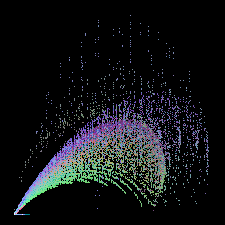
\includegraphics[width=1\textwidth]{gradient_intensity_spatial.png}
		\caption{A plot of gradient and intensity with colour coded spatial position}
		\label{fig:gradient_intensity_spatial}
	\end{minipage}~
	\begin{minipage}{.24\textwidth}
		\centering
		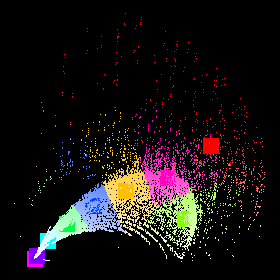
\includegraphics[width=1\textwidth]{intensity_gradient_second_derivative.png}
		\caption{The nucleon data is classified into 8 clusters with k-means. The squares represent the cluster centres. (x-axis for intensity, y-axis for gradient magnitude and z-axis for second order derivative magnitude)}
		\label{fig:intensity_gradient_second_derivative}
	\end{minipage}~
	\begin{minipage}{.24\textwidth}
		\centering
		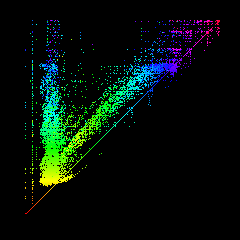
\includegraphics[width=\textwidth]{lh_histogram.png}
		\caption{LH histogram with colour coded intensity (x-axis for L values and y-axis for H values)}
		\label{fig:lh_histogram}
	\end{minipage}
	%\begin{minipage}{.24\textwidth}
	%        \centering
	%        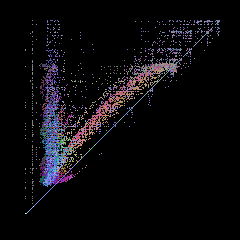
\includegraphics[width=\textwidth]{lh_histogram_spatial.png}
	%        \caption{LH histogram with colour coded spatial position}
	%        \label{fig:lh_histogram_spatial}
	%\end{minipage}
\end{figure}

%\begin{figure}
%\centering
%\begin{subfigure}[b]{0.33\textwidth}
%        \centering
%        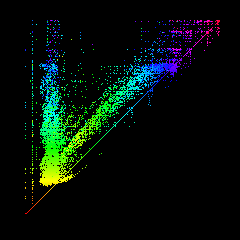
\includegraphics[width=\textwidth]{lh_histogram.png}
%        \caption{LH histogram with colour coded intensity}
%        \label{fig:lh_histogram}
%\end{subfigure}%
%~ %add desired spacing between images, e. g. ~, \quad, \qquad etc.
%  %(or a blank line to force the subfigure onto a new line)
%\begin{subfigure}[b]{0.33\textwidth}
%        \centering
%        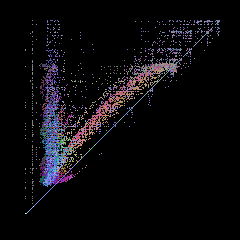
\includegraphics[width=\textwidth]{lh_histogram_spatial.png}
%        \caption{LH histogram with colour coded spatial position}
%        \label{fig:lh_histogram_spatial}
%\end{subfigure}
%\caption{LH histogram}\label{fig:lh_histogram_images}
%\end{figure}

\subsection{Results}
The contour outlining approach described in this section is an image space addition to volume rendering. In this approach, the layers used for edge detection is rendered from a partial volume, which is one or more clusters from the clustering approach described above. Note how contours of different elements of the substructure are enhanced in comparison to the basic renderings in Figure~\ref{fig:Engine_spectrum_8} and Figure~\ref{fig:VisMale_spectrum_4}.

Figure~\ref{fig:Engine_spectrum_8} shows an image rendered from the Engine block data set with a generated transfer function (8 sets of evenly distributed control points). First, we performed a global optimization on the transfer function (Figure~\ref{fig:Engine_spectrum_8_balance_1000}), then the voxels are classified into 8 clusters by the k-means clustering based on voxel intensities, gradient magnitudes and second derivatives. Figure~\ref{fig:Engine_spectrum_8_balance_1000_cluster_1_of_8} and Figure~\ref{fig:Engine_spectrum_8_balance_1000_cluster_7_of_8} display two of the 8 clusters. The two clusters are rendered; then edge detection is performed respectively and the resulting contours are shown in Figure~\ref{fig:Engine_spectrum_8_balance_1000_cluster_1_of_8_contour} and Figure~\ref{fig:Engine_spectrum_8_balance_1000_cluster_7_of_8_contour}. Finally, the contours are blended with the previous rendered image, as displayed in Figure~\ref{fig:Engine_spectrum_8_balance_1000_cluster_1_of_8_contour_combined} and Figure~\ref{fig:Engine_spectrum_8_balance_1000_cluster_7_of_8_contour_combined}.



\begin{figure}
	\centering
	\begin{minipage}{.24\textwidth}
		\centering
		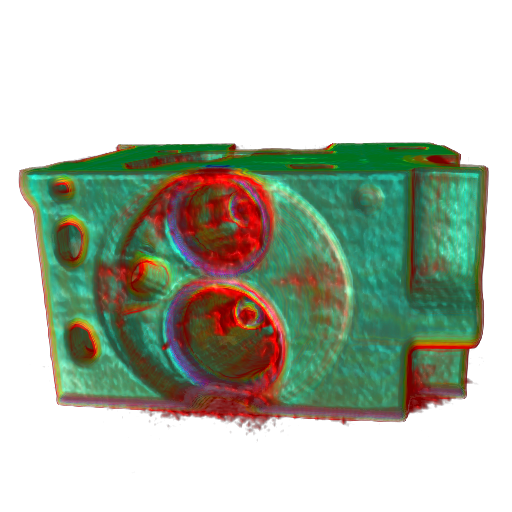
\includegraphics[width=\textwidth]{Engine_spectrum_8.png}
		\caption{Before transfer function optimization}
		\label{fig:Engine_spectrum_8}
	\end{minipage}~
	%\begin{minipage}{.24\textwidth}
	%        \centering
	%        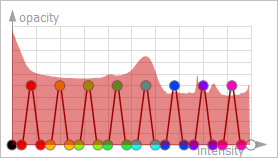
\includegraphics[width=\textwidth]{tf_Engine_spectrum_8.png}
	%        \caption{}
	%        \label{fig:tf_Engine_spectrum_8}
	%\end{minipage}~
	\begin{minipage}{.24\textwidth}
		\centering
		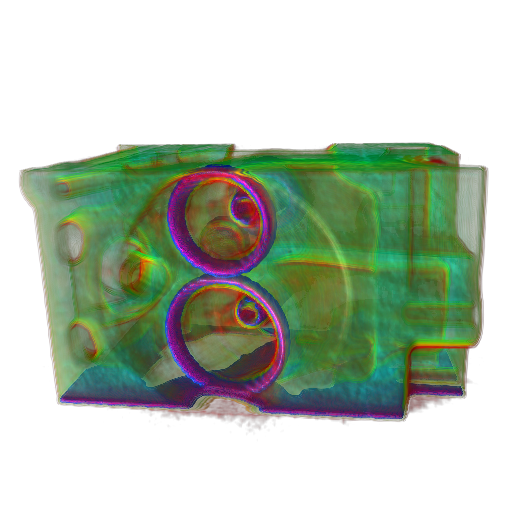
\includegraphics[width=\textwidth]{Engine_spectrum_8_balance_1000.png}
		\caption{After transfer function optimization}
		\label{fig:Engine_spectrum_8_balance_1000}
	\end{minipage}~
	%\begin{minipage}{.24\textwidth}
	%        \centering
	%        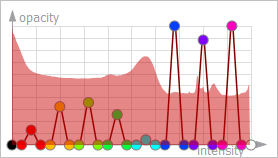
\includegraphics[width=\textwidth]{tf_Engine_spectrum_8_balance_1000.png}
	%        \caption{}
	%        \label{fig:tf_Engine_spectrum_8_balance_1000}
	%\end{minipage}
	\begin{minipage}{.24\textwidth}
		\centering
		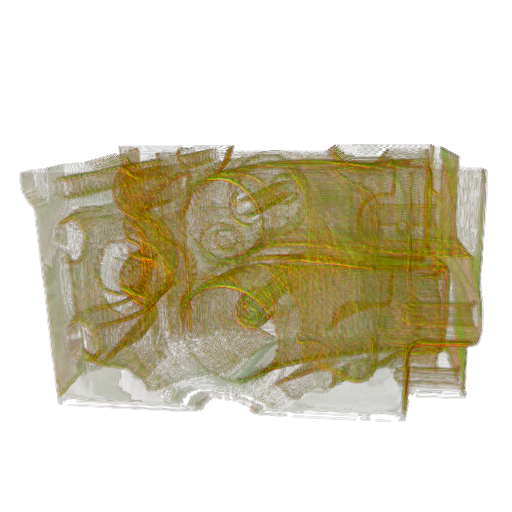
\includegraphics[width=\textwidth]{Engine_spectrum_8_balance_1000_cluster_1_of_8.png}
		\caption{A cluster of the volume}
		\label{fig:Engine_spectrum_8_balance_1000_cluster_1_of_8}
	\end{minipage}~
	\begin{minipage}{.24\textwidth}
		\centering
		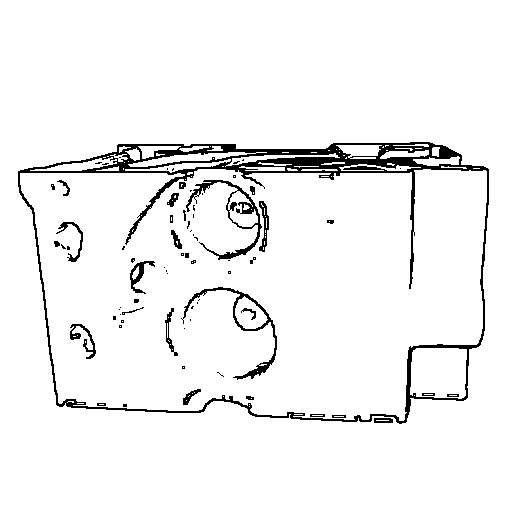
\includegraphics[width=\textwidth]{Engine_spectrum_8_balance_1000_cluster_1_of_8_contour.png}
		\caption{Edge detection is performed on the cluster}
		\label{fig:Engine_spectrum_8_balance_1000_cluster_1_of_8_contour}
	\end{minipage}
	\begin{minipage}{.24\textwidth}
		\centering
		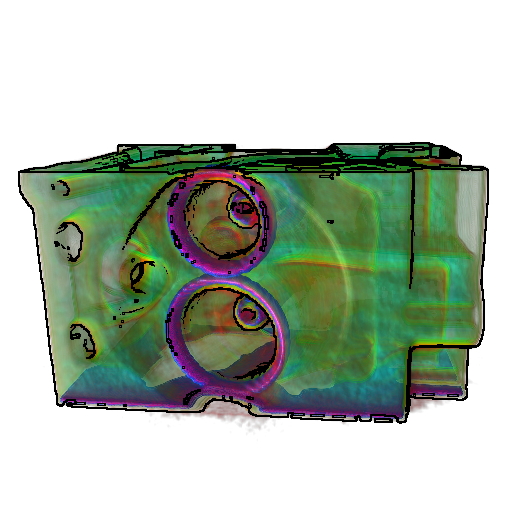
\includegraphics[width=\textwidth]{Engine_spectrum_8_balance_1000_cluster_1_of_8_contour_combined.png}
		\caption{The contour is blended with \ref{fig:Engine_spectrum_8_balance_1000}. Contours of the outside shapes are enhanced.}
		\label{fig:Engine_spectrum_8_balance_1000_cluster_1_of_8_contour_combined}
	\end{minipage}~
	\begin{minipage}{.24\textwidth}
		\centering
		
\includegraphics[width=\textwidth]{Engine_spectrum_8_balance_1000_cluster_7_of_8.png}
		\caption{Another cluster of the volume}
		\label{fig:Engine_spectrum_8_balance_1000_cluster_7_of_8}
	\end{minipage}~
	\begin{minipage}{.24\textwidth}
		\centering
		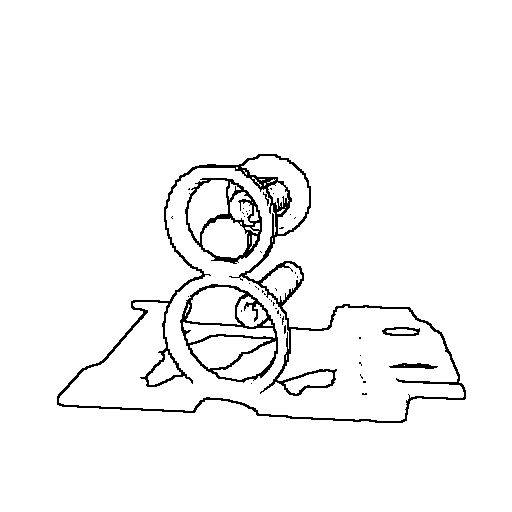
\includegraphics[width=\textwidth]{Engine_spectrum_8_balance_1000_cluster_7_of_8_contour.png}
		\caption{Edge detection is performed on the cluster}
		\label{fig:Engine_spectrum_8_balance_1000_cluster_7_of_8_contour}
	\end{minipage}~
	\begin{minipage}{.24\textwidth}
		\centering
		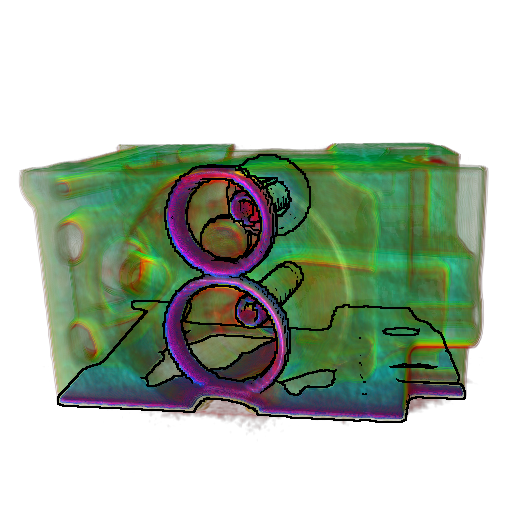
\includegraphics[width=\textwidth]{Engine_spectrum_8_balance_1000_cluster_7_of_8_contour_combined.png}
		\caption{The contour is blended with \ref{fig:Engine_spectrum_8_balance_1000}. Contours of the substructure are enhanced.}
		\label{fig:Engine_spectrum_8_balance_1000_cluster_7_of_8_contour_combined}
	\end{minipage}
\end{figure}

Another set of results are obtained from the VisMale data set. First, the data set is rendered with a generated transfer function (4 sets of evenly distributed control points), as shown in Figure~\ref{fig:VisMale_spectrum_4}. Then the transfer function is optimized (Figure~\ref{fig:VisMale_spectrum_4_balance_1000}). Two clusters are rendered respectively (Figure~\ref{fig:VisMale_spectrum_4_balance_1000_cluster_2_of_8} and Figure~\ref{fig:VisMale_spectrum_4_balance_1000_cluster_5_of_8}), and edge detection is performed to obtain the contours (Figure~\ref{fig:VisMale_spectrum_4_balance_1000_cluster_2_of_8_contour} and Figure~\ref{fig:VisMale_spectrum_4_balance_1000_cluster_5_of_8_contour}). Finally, the contours are blended back to the previous rendered image (Figure~\ref{fig:VisMale_spectrum_4_balance_1000_cluster_2_of_8_contour_combined} and Figure~\ref{fig:VisMale_spectrum_4_balance_1000_cluster_5_of_8_contour_combinedpectrum_4}).

\pagebreak

\begin{figure}
	\centering
	\begin{minipage}{.24\textwidth}
		\centering
		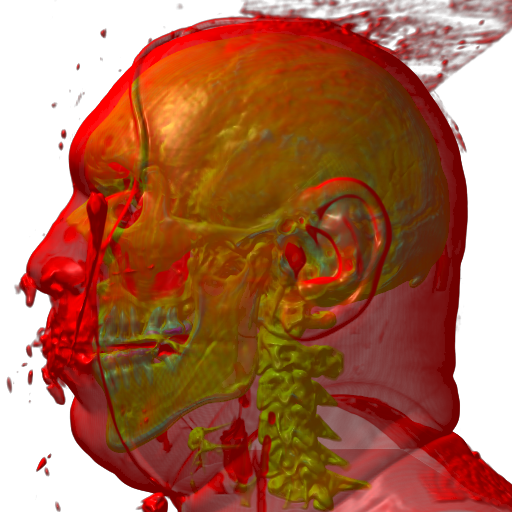
\includegraphics[width=1\textwidth]{VisMale_spectrum_4.png}
		\caption{Before transfer function optimization}
		\label{fig:VisMale_spectrum_4}
	\end{minipage}~
	\begin{minipage}{.24\textwidth}
		\centering
		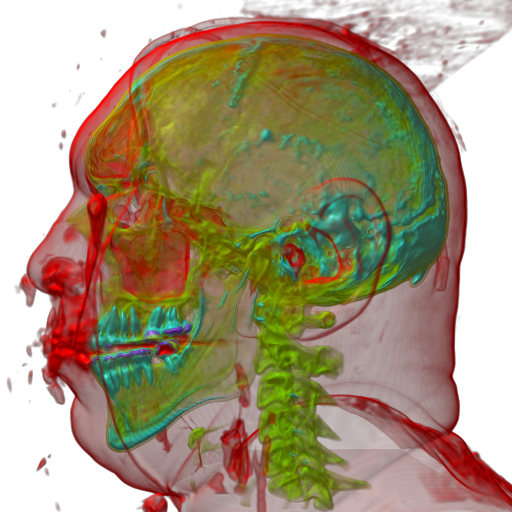
\includegraphics[width=1\textwidth]{VisMale_spectrum_4_balance_1000.png}
		\caption{After transfer function optimization}
		\label{fig:VisMale_spectrum_4_balance_1000}
	\end{minipage}~
	\begin{minipage}{.24\textwidth}
		\centering
		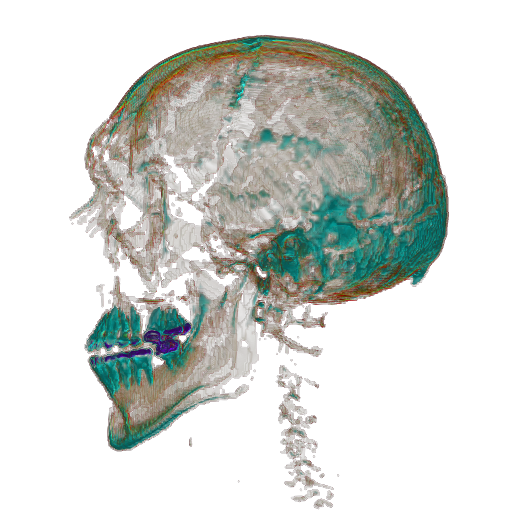
\includegraphics[width=1\textwidth]{VisMale_spectrum_4_balance_1000_cluster_2_of_8.png}
		\caption{A cluster of the volume}
		\label{fig:VisMale_spectrum_4_balance_1000_cluster_2_of_8}
	\end{minipage}~
	\begin{minipage}{.24\textwidth}
		\centering
		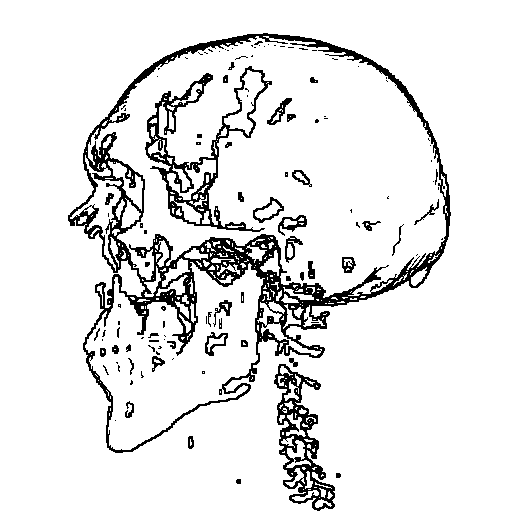
\includegraphics[width=1\textwidth]{VisMale_spectrum_4_balance_1000_cluster_2_of_8_contour.png}
		\caption{Edge detection is performed on the cluster}
		\label{fig:VisMale_spectrum_4_balance_1000_cluster_2_of_8_contour}
	\end{minipage}
	\begin{minipage}{.24\textwidth}
		\centering
		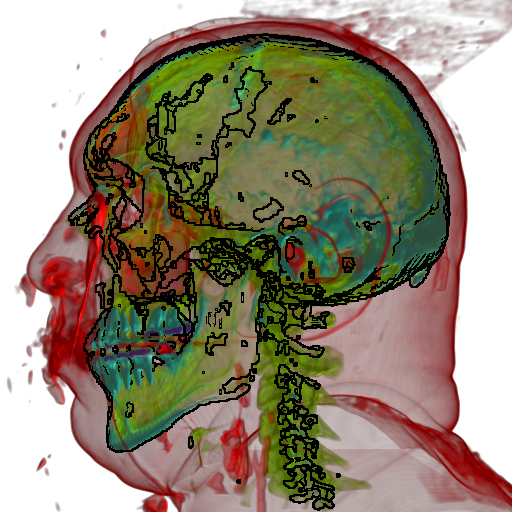
\includegraphics[width=1\textwidth]{VisMale_spectrum_4_balance_1000_cluster_2_of_8_contour_combined.png}
		\caption{The contour is blended with \ref{fig:VisMale_spectrum_4_balance_1000}. Contours of the substructure are enhanced.}
		\label{fig:VisMale_spectrum_4_balance_1000_cluster_2_of_8_contour_combined}
	\end{minipage}~
	\begin{minipage}{.24\textwidth}
		\centering
		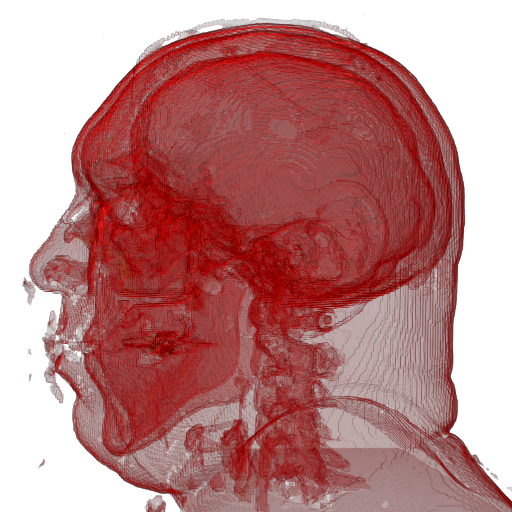
\includegraphics[width=1\textwidth]{VisMale_spectrum_4_balance_1000_cluster_5_of_8.png}
		\caption{Another cluster of the volume}
		\label{fig:VisMale_spectrum_4_balance_1000_cluster_5_of_8}
	\end{minipage}~
	\begin{minipage}{.24\textwidth}
		\centering
		\includegraphics[width=1\textwidth]{VisMale_spectrum_4_balance_1000_cluster_5_of_8_contour.png}
		\caption{Edge detection is performed on the cluster}
		\label{fig:VisMale_spectrum_4_balance_1000_cluster_5_of_8_contour}
	\end{minipage}~
	\begin{minipage}{.24\textwidth}
		\centering
		\includegraphics[width=1\textwidth]{VisMale_spectrum_4_balance_1000_cluster_5_of_8_contour_combined.png}
		\caption{The contour is blended with \ref{fig:VisMale_spectrum_4_balance_1000}. Contours of the outside shapes are enhanced.}
		\label{fig:VisMale_spectrum_4_balance_1000_cluster_5_of_8_contour_combinedpectrum_4}
	\end{minipage}
\end{figure}


%-------------------------------------------------------------------------
